\documentclass[10pt,twocolumn,letterpaper]{article}

\usepackage{cvpr}
\usepackage{times}
\usepackage{epsfig}
\usepackage{graphicx}
\usepackage{caption}
\usepackage{subcaption}
\usepackage{amsmath}
\usepackage{amssymb}

% Include other packages here, before hyperref.

% If you comment hyperref and then uncomment it, you should delete
% egpaper.aux before re-running latex.  (Or just hit 'q' on the first latex
% run, let it finish, and you should be clear).
%\usepackage[pagebackref=true,breaklinks=true,letterpaper=true,colorlinks,bookmarks=false]{hyperref}

\cvprfinalcopy % *** Uncomment this line for the final submission

\def\cvprPaperID{****} % *** Enter the CVPR Paper ID here
\def\httilde{\mbox{\tt\raisebox{-.5ex}{\symbol{126}}}}

% Pages are numbered in submission mode, and unnumbered in camera-ready
%\ifcvprfinal\pagestyle{empty}\fi
\setcounter{page}{1}
\begin{document}

%%%%%%%%% TITLE
\title{Classification by Committee: \\ Labeling Marine Life Using an Ensemble of Experts}

%\author{Steven Hickson, Andrew Price \\
%Georgia Institute of Technology\\
%{\tt\small me@stevenhickson.com, arprice@gatech.edu}
%}

\author{Team 3}

\maketitle
%\thispagestyle{empty}


%%%%%%%%% BODY TEXT
\section{Introduction}
 Classification of elements in images has been a major topic in computer vision for a long time, due to its high degree of both difficulty and utility.
 One such application of object classification has been automated recognition of marine species.
 The ability to automatically identify species in an image would prove highly useful to both academic pursuits (eg. species surveying for a coral reef) and educational audiences (eg. a guided aquarium tour program).
 
 In this work, we present preliminary results showing how a committee of expert systems can be leveraged to provide reasonably high matching rates while maintaining low incidences of false positives. Results are shown for data captured by hand at the Georgia Aquarium and acquired online.

\section{Related Work}
 Much work on classifying fish species has been done in highly controlled environments, usually requiring a carefully selected background and fish orientation \cite{white2006automated}.
 These approaches often require additional specialized equipment such as laser scanners or conveyor belts \cite{storbeck2001fish}, or require species dependent domain knowledge \cite{thonnat1988expert}.
  
  Our approach will differ from the related techniques in a number of important ways.
  First, animals are being classified in a semi-structured environment, meaning that while we may not have full control over the pose and context of a sample image, there are a limited set of species to choose from and a finite set of backgrounds and scenes.
  Second, we will rely on a variety of image features, along the lines presented in \cite{berg2006animals}, but we will not incorporate text clues into the classifier.

\section{Implementation}
  The first stage in building an ensemble classifier is the training (and evaluation) of the individual expert systems. For this purpose, we implemented and tested a number of individual classifiers using a variety of features before settling on a final configuration. In order to realize major performance improvements, the various classifiers of an ensemble need to be diverse in both their training data and their classification method \cite{rokach2010ensemble}. Therefore, we experimented with SURF \cite{bay2006surf} and ORB \cite{rublee2011orb} feature detectors and descriptors for capturing texture patches, HoGs \cite{dalal2005histograms} for overall shape, and colored histograms \cite{stricker1995similarity} for HSV color similarity. For the point features, we used a bag of words \cite{csurka2004visual} fed into an SVM classifier. The histogram features were compared using both correlation and Bhattacharyya \cite{bhattacharyya1943distance} distance.
  
  Of all of these feature vectors and classifiers, the SURF features and color histograms provided the best matching performance, and, more importantly, failed to agree on false positive matches. 
  
  In order to train this system, we provided three sets of images: template images to give the bag of words a suitable vocabulary, labeled training images, and unlabeled testing images. In a number of test sets, all of these images were captured with a single camera during a visit to the Aquarium. In other test runs, these images were augmented with representative images drawn from the Internet.

\section{Evaluation}
We plan to evaluate the classifier performance by generating a confusion matrix based on images drawn from a large subset of the species living at the Atlanta Aquarium. 
Additionally, we will compare the performance of the aggregated features against classifiers based on the individual features.
Finally, we will be comparing against \cite{berg2006animals} to determine the degree of dependency on text information.
We expect the concatenated features to outperform in situations where marine life shares a similar environment, and therefore shares similar color or shape characteristics.

\begin{figure*}[ht]
\begin{center}
	\begin{subfigure}[b]{0.24\linewidth}
		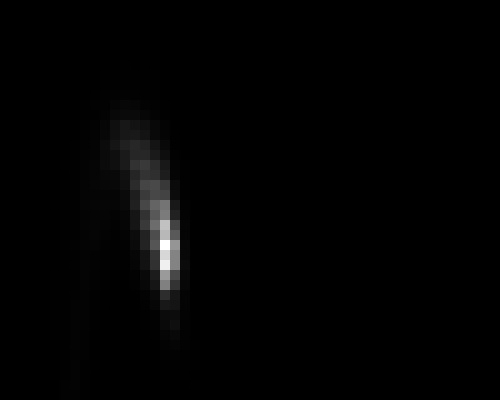
\includegraphics[width=\textwidth]{Angelfish_hist.jpg}
		\caption{Fusiliers}
	\end{subfigure}
	\begin{subfigure}[b]{0.24\linewidth}
		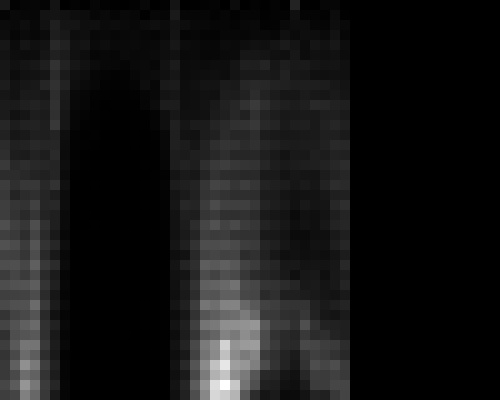
\includegraphics[width=\textwidth]{Jellyfish_hist.jpg}
		\caption{Jellyfish}
	\end{subfigure}
	\begin{subfigure}[b]{0.24\linewidth}
		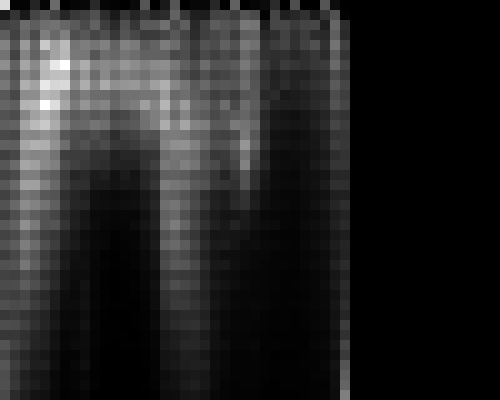
\includegraphics[width=\textwidth]{PointyFish_hist.jpg}
		\caption{Lionfish}
	\end{subfigure}
	\begin{subfigure}[b]{0.24\linewidth}
		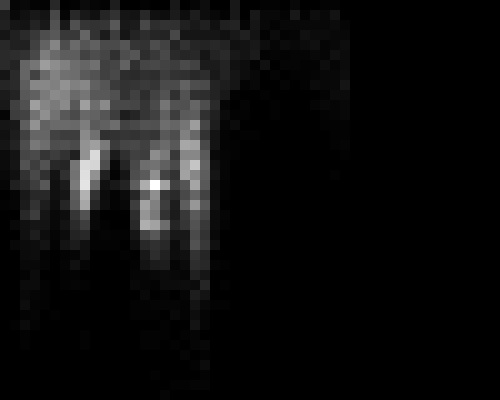
\includegraphics[width=\textwidth]{current_hist.jpg}
		\caption{Query Image}
	\end{subfigure}

\end{center}
\caption{\small A sample of 2D color histograms with a query image.}
\label{fig:colorHists}
\end{figure*}



\section{Discussion}
	In our experiments, the performance of the classifier was highly dependent on the number and quality of training images. While this may seem obvious on first inspection, the classifier was sensitive to the point of near instability to certain images in the training set. This is likely due to the relatively small size of our training set ($<$ 100 images), and to the fact that only 2 sets of features were used.
	
	A second improvement would be the application of a more rigorous voting scheme. In its current state, both experts are considered equally valid over all query images. However, our experiments revealed that certain features were more discriminative than others under certain viewing conditions. (For instance, animals in the same tank tend to have similar color histograms.) This could be resolved by using voting weights derived from both the historical accuracy of a classifier for a particular class and from the confidence value for a given query image.
	
	A final opportunity for future work would be the incorporation of a region of interest (ROI) over the input images. For the most part, the subject of interest tends to fall within the middle third of both training and query images, so these regions could be given higher weights. This would likely help differentiate images in which multiple species are present, but may reduce the benefit of context clues such as background scenery.

\begin{figure*}[ht]
\begin{center}
	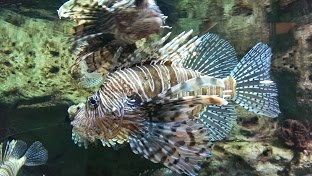
\includegraphics[width=0.21\linewidth]{1_input.jpg}
	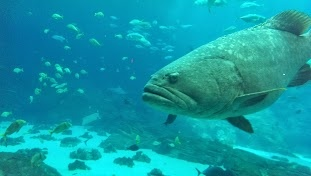
\includegraphics[width=0.21\linewidth]{2_input.jpg}
	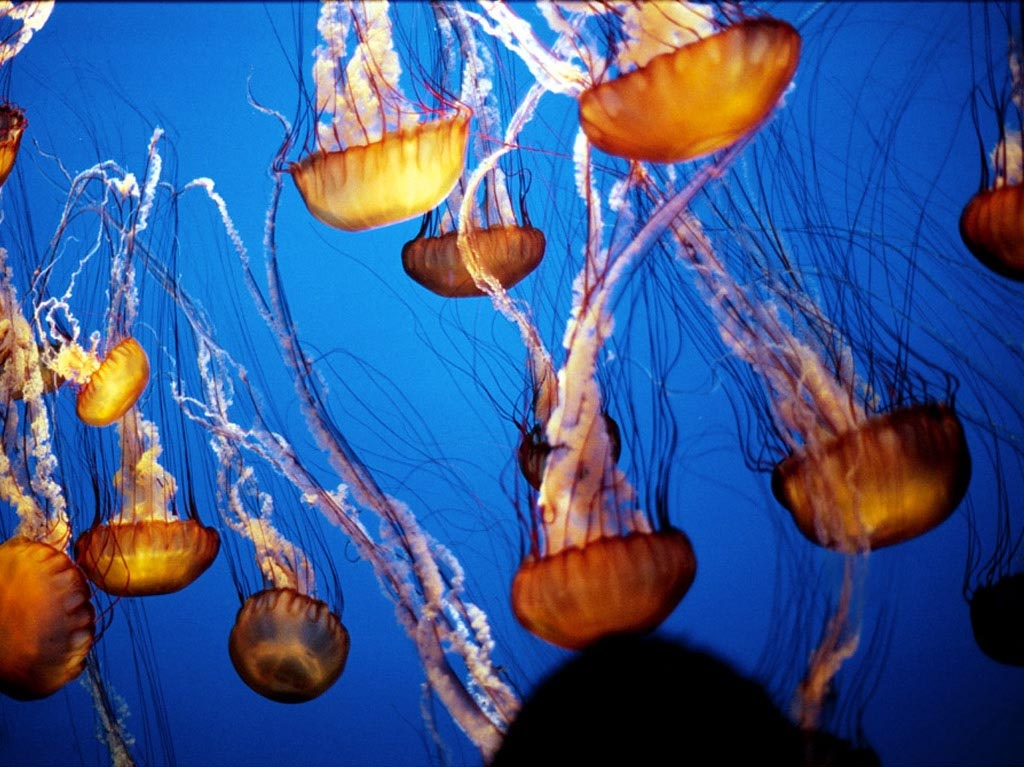
\includegraphics[width=0.21\linewidth]{3_input.jpg}
	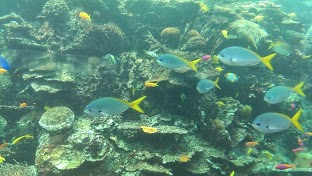
\includegraphics[width=0.21\linewidth]{4_input.jpg}
	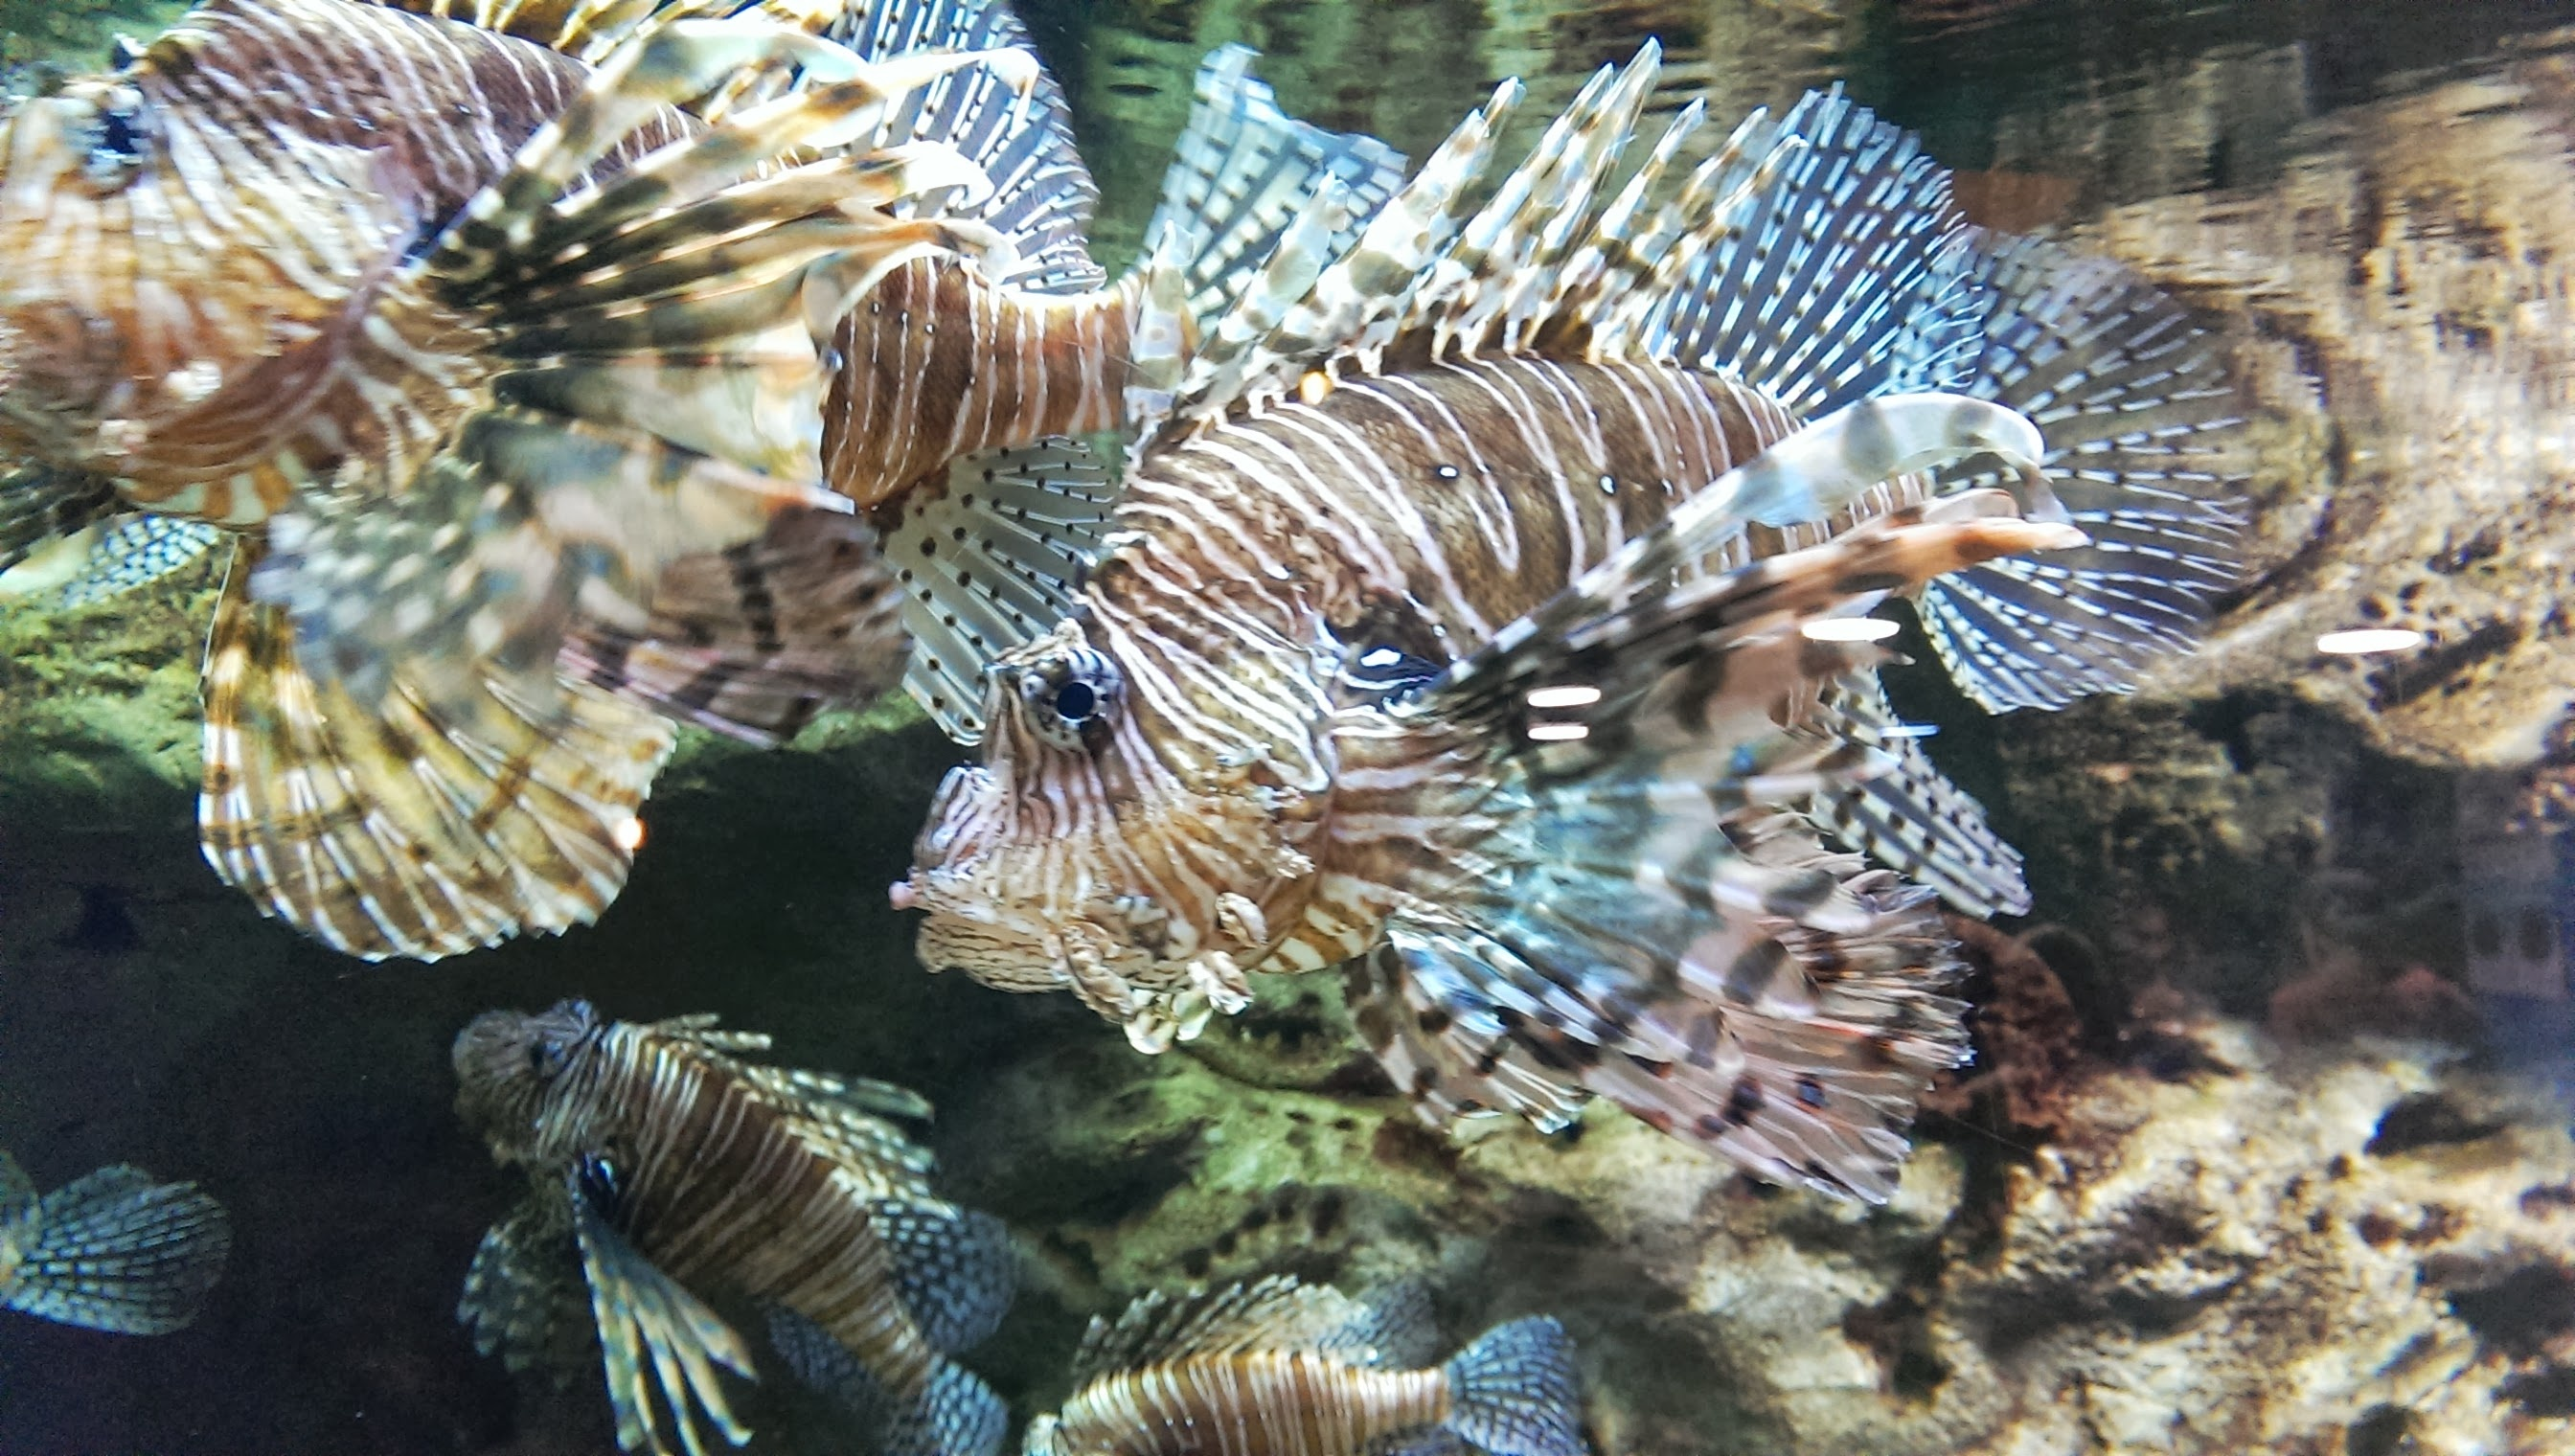
\includegraphics[width=0.21\linewidth]{1_output.jpg}
	~
	~
	~
	~
	~
	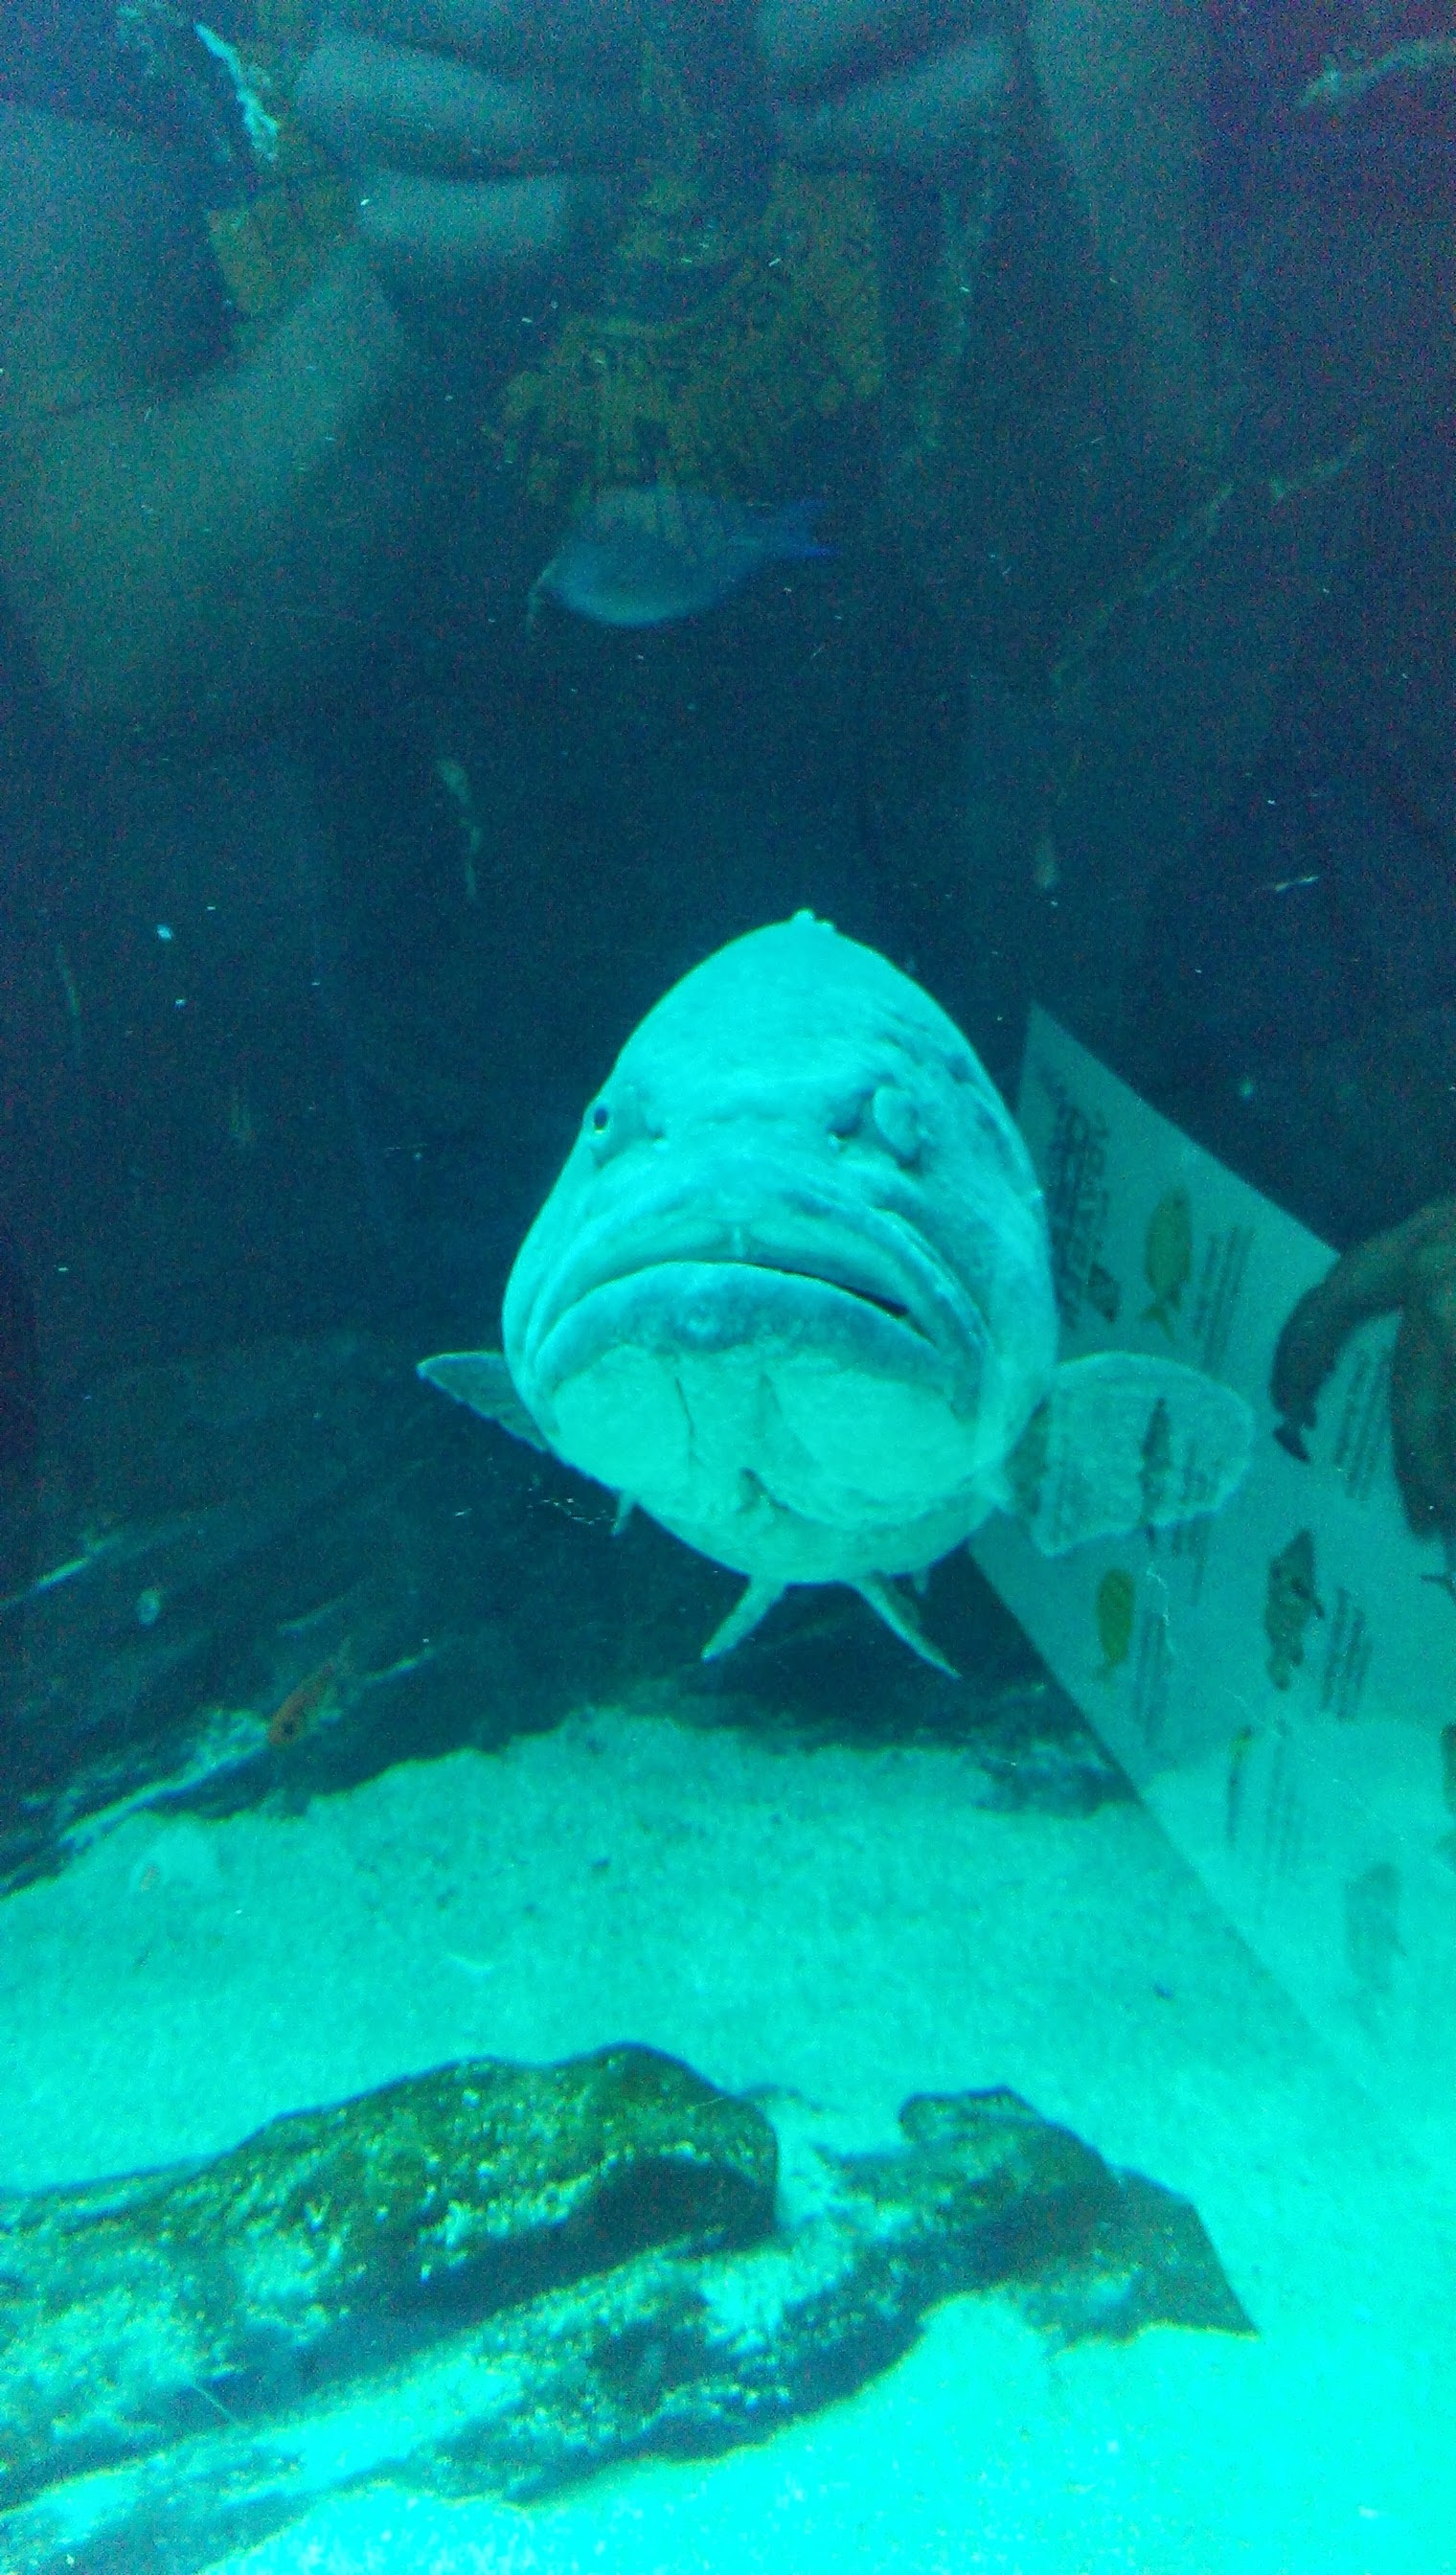
\includegraphics[width=0.10\linewidth]{2_output.jpg}
	~
	~
	~
	~
	~
	~
	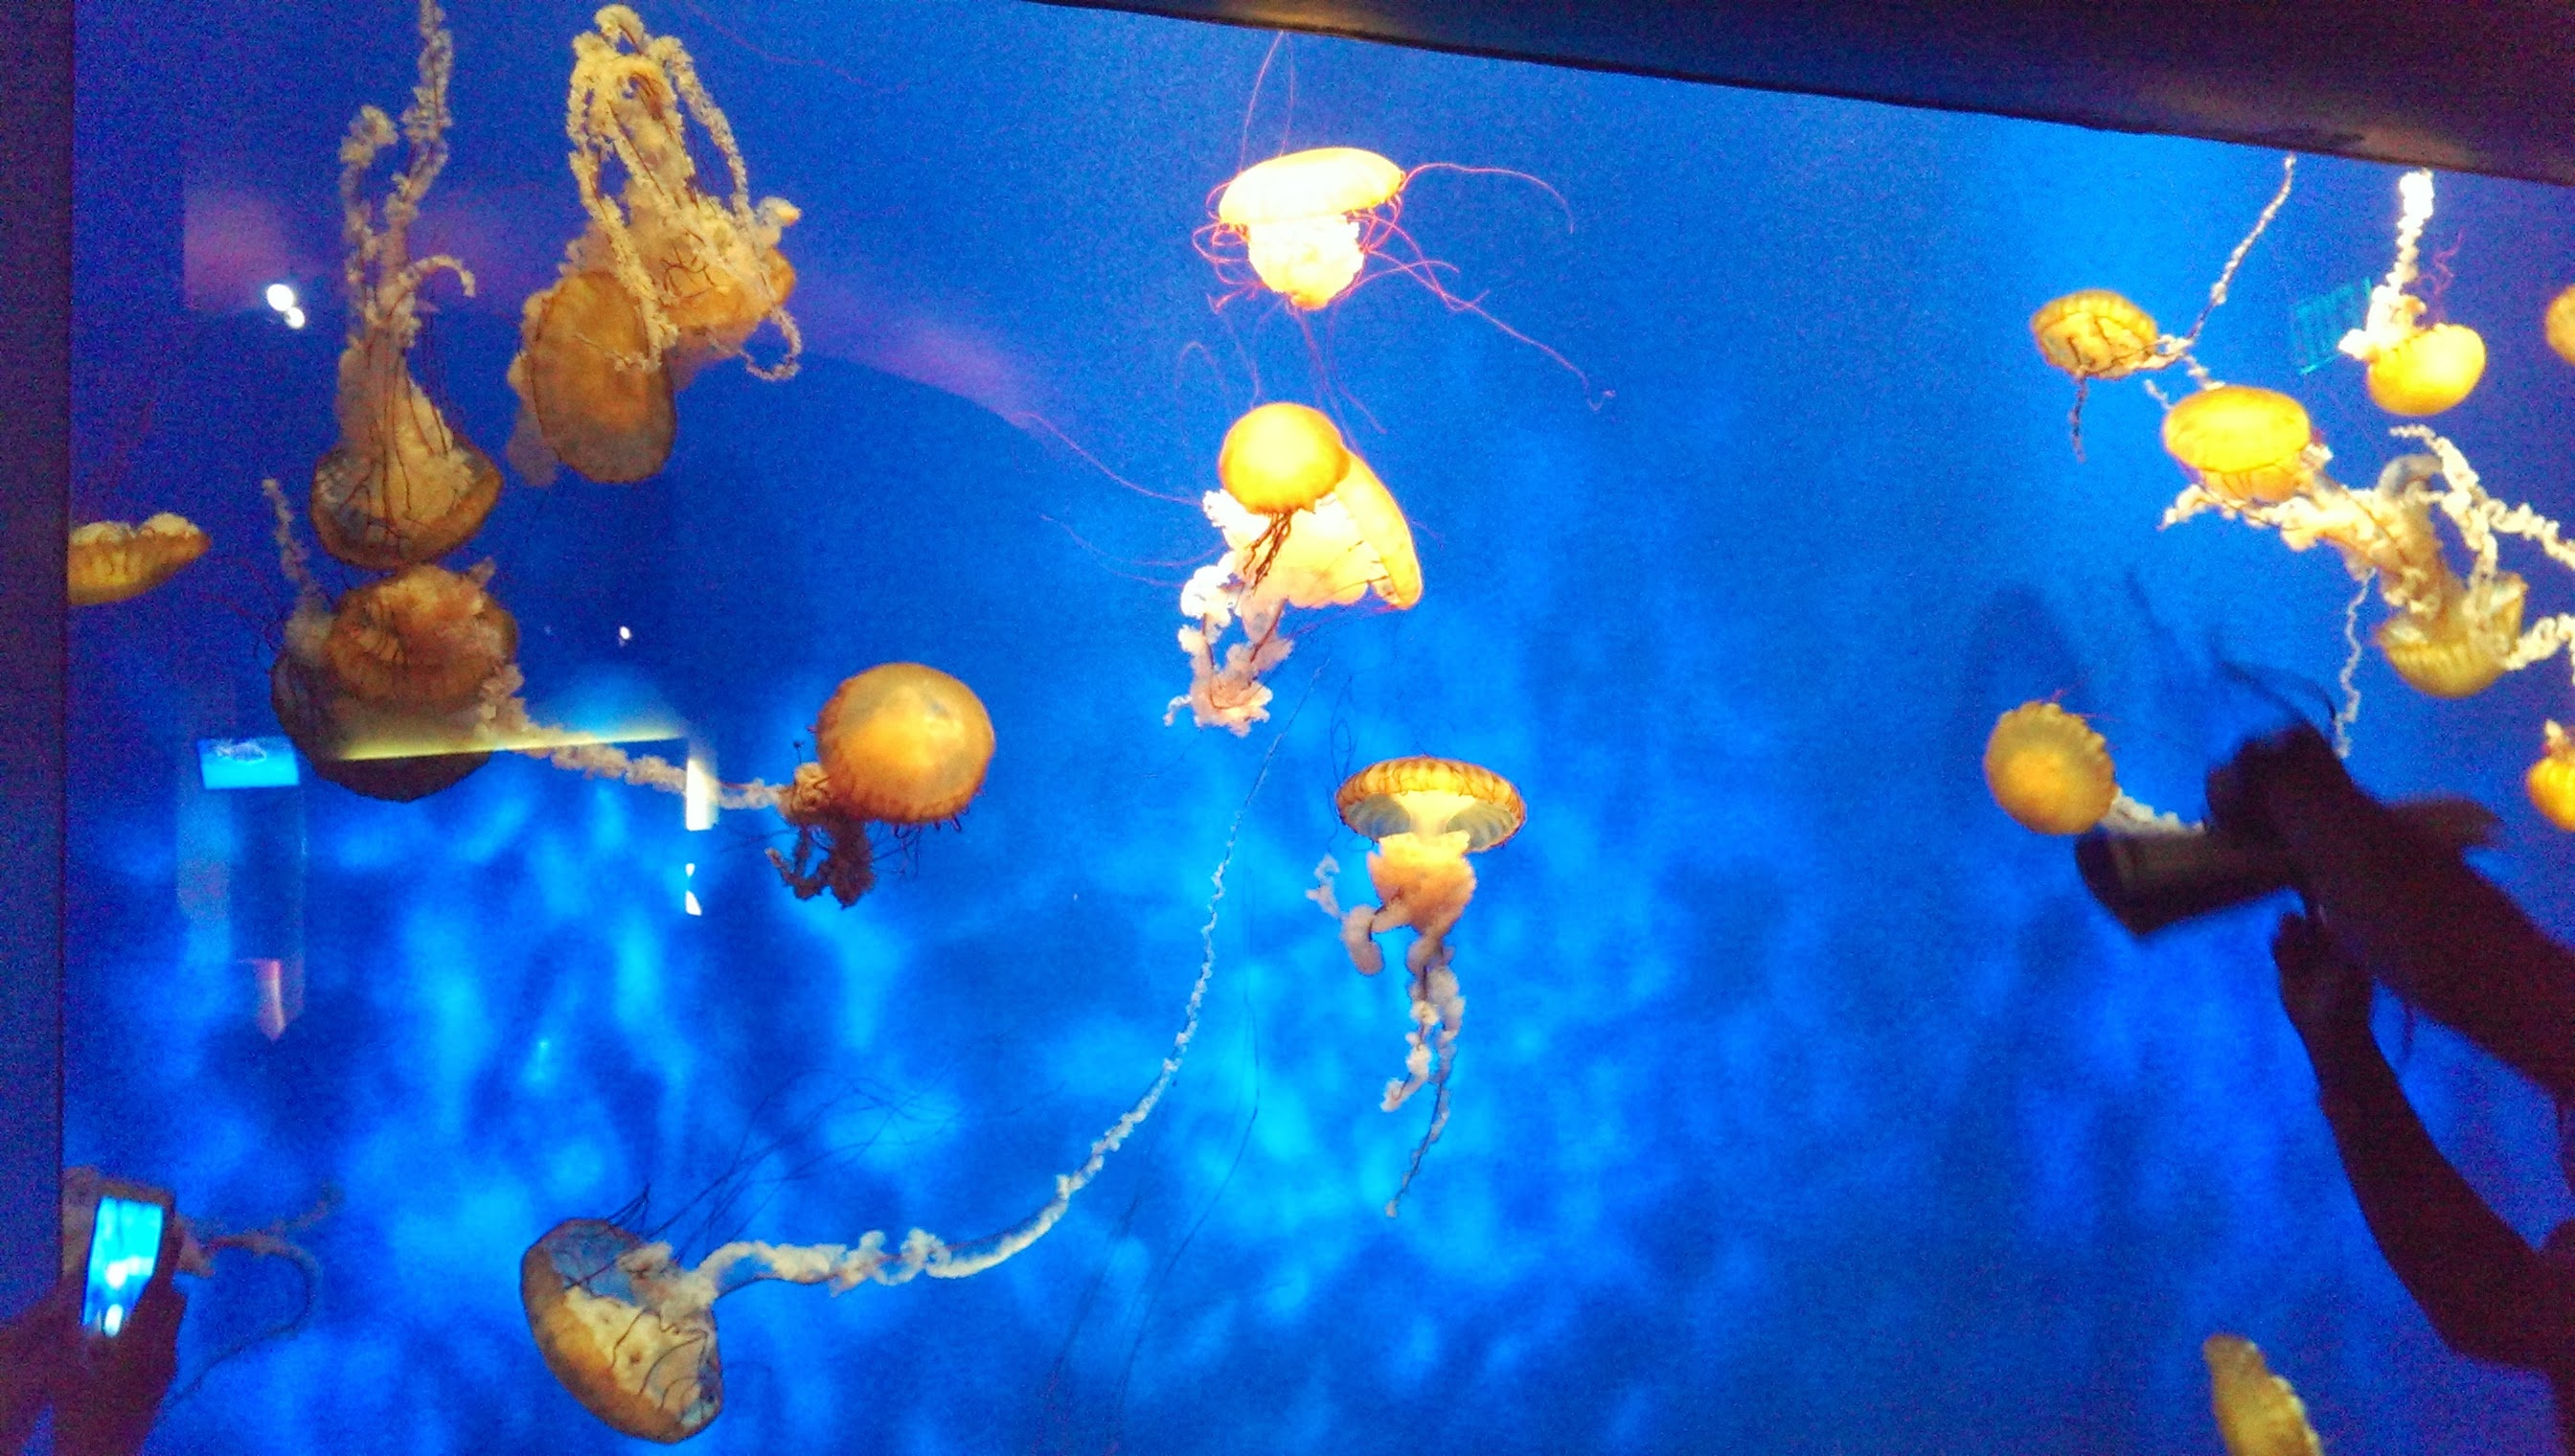
\includegraphics[width=0.21\linewidth]{3_output.jpg}
	
\includegraphics[width=0.21\linewidth]{4_output.jpg}
\end{center}
\caption{\small A sample of correctly matched images with an unsuccessfully matched image.}
\label{fig:matchResults}
\end{figure*}


%-------------------------------------------------------------------------

{\small
\bibliographystyle{unsrt}
\bibliography{egbib}
}

\end{document}
